 %%%%%%%%%%%%%%%%%%%%%%%%%%%%%%%%%%%%%%%%%
% Beamer Presentation
% LaTeX Template
% Version 1.0 (10/11/12)
%
% This template has been downloaded from:
% http://www.LaTeXTemplates.com
%
% License:
% CC BY-NC-SA 3.0 (http://creativecommons.org/licenses/by-nc-sa/3.0/)
%
%%%%%%%%%%%%%%%%%%%%%%%%%%%%%%%%%%%%%%%%%

%----------------------------------------------------------------------------------------
%	PACKAGES AND THEMES
%----------------------------------------------------------------------------------------

\documentclass{beamer}

\mode<presentation> {
\usetheme[secheader]{Madrid}
\usecolortheme{seahorse}
\useinnertheme{circles}
}

\usepackage{graphicx} % Allows including images
\usepackage{booktabs} % Allows the use of \toprule, \midrule and \bottomrule in tables
\usepackage{tikz}
\usepackage{caption}
\usepackage{hyperref}



%----------------------------------------------------------------------------------------
%	TITLE PAGE
%----------------------------------------------------------------------------------------



\title[Designing HCI Experiments]{Designing HCI Experiments} % The short title appears at the bottom of every slide, the full title is only on the title page

\author{Chaklam Silpasuwanchai} % Your name
\institute[AIT] % Your institution as it will appear on the bottom of every slide, may be shorthand to save space
{
Asian Institute of Technology \\ % Your institution for the title page
\medskip
\textit{chaklam@ait.asia} % Your email address
}
\date{} % Date, can be changed to a custom date

\AtBeginSection[]
{
\begin{frame}<beamer> 
\tableofcontents[currentsection]  % show TOC and highlight current section
\end{frame}
}

\begin{document}

\begin{frame}
\titlepage % Print the title page as the first slide
\end{frame}

\begin{frame}
\frametitle{Overview} % Table of contents slide, comment this block out to remove it
\tableofcontents
 % Throughout your presentation, if you choose to use \section{} and \subsection{} commands, these will automatically be printed on this slide as an overview of your presentation
\end{frame}

%----------------------------------------------------------------------------------------
%	PRESENTATION SLIDES
%----------------------------------------------------------------------------------------

\begin{frame}
\frametitle{Sources} 
\begin{itemize}
	\item Mackenzie, Chapter 4-5, \textbf{Scientific Foundations, Designing HCI Experiments},  Human Computer Interaction: An Empirical Research Perspective, 1st ed. (2013) 
	\item Zhao, \textbf{How to Design Controlled Experiments in HCI?} \url{https://www.slideshare.net/shilman/controlled-experiments-shengdong-zhao}
\end{itemize}
\end{frame}


%------------------------------------------------
%\section{Scientific Foundations} % Sections can be created in order to organize your presentation into discrete blocks, all sections and subsections are automatically printed in the table of contents as an overview of the talk
%-----------------------------------------------


%\begin{frame}
%	\frametitle{Reminders}
%	\begin{itemize}
%		\item \textbf{Team forming} %due this Friday
%		\item \textbf{Project} - starts reading CHI 2020 - 2021 papers!  And make sure to check all the deadlines in Google Classroom
%	\end{itemize}
%\end{frame}


%\begin{frame}
%	\frametitle{Reminders} % Table of contents slide, comment this block out to remove it
%	\begin{itemize}
%		\item  First draft of proposal due soon.  Hard and soft copies as usual.
%	\end{itemize}
%\end{frame}

%\begin{frame}
%	\frametitle{What is empirical research?}
%	\begin{itemize}
%		\item Empirical means \textit{originating in or based on observation or experience}.  It also means \textit{capable of being verified or disproved by observation or experiment}
%		\item Thus in HCI, empirical research is framed by \textbf{hypotheses}, where these hypotheses are verified by gathering and testing \textbf{evidence}
%		\item In a lot of sense, empirical research covers a quantifiable, observable, reproducible aspects of interaction
%	\end{itemize}
%\end{frame}

%\begin{frame}
%	\frametitle{Research Methods}
%	\begin{itemize}
%		\item \textbf{Observational} Methods - include interviews, case studies, focus groups, think-aloud protocols, and so on.  This approach is qualitative. As a result, this method achieve \textbf{relevance} while sacrificing precision.  These methods are useful for understand the reasons underlying human behavior, as opposed to \textit{what}, \textit{where}, \textit{when}
%		\item \textbf{Experimental} Methods - also called the \textit{scientific method} - knowledge is acquired through controlled experiments.  This methodology brings \textbf{precision} while sacrificing relevance.  Experimental Methods have Independent Variables and Dependent Variables
%		\item \textbf{Correlational} Methods - looks for \textbf{relationships} between variables, e.g., privacy settings vs. IQ
%	\end{itemize}
%\end{frame}


\begin{frame}
%	\footnotesize
	\frametitle{Research Methods}
	\begin{itemize}
%		\item Allen Newell did not hesitate: ``\textit{Science is method. Everything else is commentary.}" If the methodology is weak or flawed, there is no science forthcoming. What remains is little else than commentary.
		\item In HCI research, the most accepted method is \textbf{experimental method}.  %Of course, it is clear that experimental method will often include observational methods and correlational methods
		\item \textbf{Golden rule} is 70\% quantitative (verification of effects) and 30\% qualitative (tell us why)
		\item In experimental research, \textbf{comparative evaluation} is often done, where \textbf{proposed solution} is pit against (1) \textbf{state-of-the art} technique and (2) \textbf{baseline} technique.  
		\begin{itemize}
			\item Baseline allows comparison of results with past studies.  State-of-art allows comparison of proposed solution against the ``best''
		\end{itemize}
%		\item \textbf{Methodology} involves deciding the question, the \textbf{independent} and \textbf{dependent} variables, on the \textbf{participants}, the hardware and software (materials or \textbf{apparatus}), the \textbf{tasks}, the \textbf{order} of tasks, the \textbf{procedure} for briefing and preparing the participants, the \textbf{data collected and analyzed}, etc. 
%		\item So what's one appropriate methodology for research in HCI?  \textbf{Factorial experiments} - where participants are exposed to levels of factors while their performance is observed and measured
	\end{itemize}
\end{frame}

%\begin{frame}
%\frametitle{Comparative Evaluations}
%\begin{figure}
%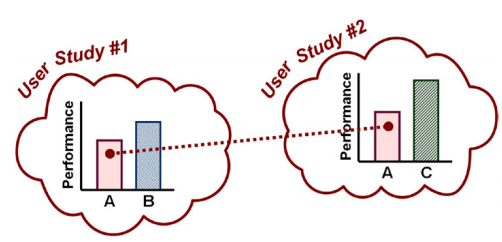
\includegraphics[width=0.9\linewidth]{baseline}
%\caption{Source: Fg. 4.10 (Mackenzie)}
%\end{figure}
%\end{frame}

%\begin{frame}
%	\frametitle{Observe and Measure}
%	\begin{itemize}
%		\item Observation alone is of limited value.  
%		\item There are four scales of measurement: nominal, ordinal, interval, and ratio
%		\item We need to know these scales in order to apply appropriate data analyses
%		\item \textbf{Nominal}: data that identify mutually exclusive categories (also known as \textit{categorical data}, e.g., M for Male, F for Female).  It is meaningless to perform mathematical manipulations on nominal data.  Usually work with count or frequency (e.g., how many males do X).  Nominal variables are usually our independent variables or variables used in correlational study
%		\item \textbf{Ordinal}: provide an order or ranking.  It is possible to perform comparison of ordinal data but \textbf{it is not valid to compute the mean} of ordinal data
%	\end{itemize}
%\end{frame}

%\begin{frame}
%	\frametitle{Observe and Measure}
%	\begin{itemize}
%		\item \textbf{Interval}: data that have \textbf{equal distances between adjacent values} but with no absolute zero, e.g., Temperature, Likert-Scale.  It is meaningful to compute mean of interval data (e.g., mean temperature now is X Celsius).  However, it is not meaningful to compute the \textbf{ratio} of interval data (e.g., one cannot say 20 Celsius is twice as warm as 10 Celsius)
%		\item \textbf{Ratio}: data that have absolute zero and data can be added, subtracted, multiplied, divided, means, standard deviations.  Example includes distances, words per minute, time, users' age.
%		\item When we perform data analysis, it is important to use \textit{standardized, normalized metric} such as \textbf{word per minute} and \textbf{error rate}, to allow easy comparisons across multiple research works
%	\end{itemize}
%\end{frame}

\section{Designing HCI Experiments}

\subsection{Research Question}

\begin{frame}
	\frametitle{Research Question}
	\begin{itemize}
		\item  How does \textbf{pie menu} - our proposed solution - compared to \textbf{linear menu} in terms of performance?
	\end{itemize}
	\begin{figure}
		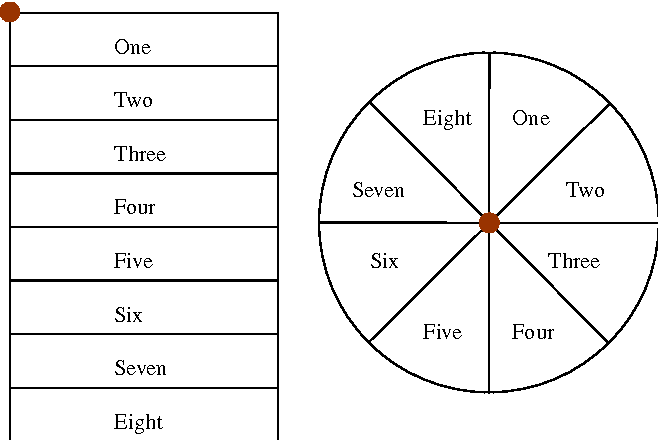
\includegraphics[width=0.6\linewidth]{pie}
		\caption{Linear menu vs. pie menu}
	\end{figure}
\end{frame}



\begin{frame}
	\footnotesize
	\frametitle{Research Question}
	"Interesting" question means (1) Not obvious, (2) Can be tested, (3) Interesting to others (not only you), (4) Make sense.
	
	\medskip	

	Are these questions "interesting"?
	\begin{itemize}
		\item What makes people happy?
		\item What causes people to like Pepsi more than Coke?
		\item Can we predict gold prices given inflation rate?
		\item Is there any preference between color preferences between male and female?
		\item Why people watches soccer more than basketball?
		\item Does taller people tend to be smarter?
		\item Does music make us happier?
		\item Does playing games increase our IQ?
		\item Why people with similar races or religion tend not to divorce?
		\item Should productivity be valued more than morals?
	\end{itemize}

\end{frame}

\begin{frame}
	\frametitle{Research Question}
	\begin{center}
		Science \textbf{cannot} answer all questions.
	\end{center}

\end{frame}

\subsection{Hypothesis}

\begin{frame}
\frametitle{Hypothesis}
\textbf{Hypothesis} is a statement containing some \textbf{educated guess.}  Why do we need to have one?  Why we just not ask the question?

\medskip

A good hypothesis is (1) specific, (2) testable, (3) has clear X and y.

\medskip

Are these good hypothesis?

\begin{itemize}
	\item Will fertilizer make my lawn grow more?
	\item Pepsi is better than coke.
	\item Studying can increase exam scores.
	\item Heat for 1 hour cause metal to expand by 10\%
	\item Dancing make us more happy than listening to music.
\end{itemize} 

All "great" research has "great" hypothesis.

\medskip

Great hypothesis comes from reading A LOT,  thinking A LOT.

\end{frame}

\begin{frame}
\frametitle{Hypothesis}

\begin{center}
All "great" research has "great" hypothesis.

\medskip

Great hypothesis comes from reading A LOT of papers, and thinking A LOT.


\end{center}
\end{frame}

\begin{frame}
\frametitle{Hypothesis}

So what's our hypothesis?

Interesting ones could be (but not limited to)

\begin{itemize}
	\item Pie menu is better than linear menu in general in terms of speed and accuracy
	\item Pie menu can be learned quickly
	\item Given small number of menu items, linear menu may perform equally to pie menu
	\item Given lots of submenus,  pie menu performance over linear menu could be even more noticeable
	\item Similarly,  pie menu performance over linear menu could be even more prominent, while walking.
\end{itemize}

\end{frame}

\subsection{Participants}

\begin{frame}
	\frametitle{Participants}
	Who should we pick?
\end{frame}

\begin{frame}
	\frametitle{Participants}
	Who should we pick?
	\begin{itemize}
		\item  Since everyone are users, we can pick anyone.  But generally, pick \textbf{target population}
		\item For statistical analysis, we will pick at least 12 participants.  A good number is around 12-15 participants.   We can also use \textbf{power analysis} or \textbf{read papers}.
	\end{itemize}
\end{frame}

\subsection{Independent Variable}

\begin{frame}
\frametitle{Independent Variables}
\begin{itemize}
	\item IV are variables we \textbf{manipulate}.  Also called \textbf{factor}. What should be our IV? 
\end{itemize}
\end{frame}

\begin{frame}
\frametitle{Independent Variables}
\begin{itemize}
	\item IV are variables we \textbf{manipulate}.  Also called \textbf{factor}.  What should be our IV?
\end{itemize}
\begin{itemize}
	\item Our first IV is the \textbf{menu type} which has two \textbf{levels}: pie menu and linear menu
	\item To increase our research generalizability, we can further adds more IV, for example:
	\begin{itemize}
		\item Second IV: \textbf{menu breadth} with 3 levels: 4, 8, 12
		\item Third IV: \textbf{menu depth} with 3 levels: 1, 2, 3
		\item Fourth IV: \textbf{usage} with 2 levels: mobile and stationary
	\end{itemize}
\end{itemize}
Thus our work is a \textbf{2 x 3 x 3 x 2 factorial design}.
\end{frame}

\begin{frame}
\frametitle{Independent Variables}
\begin{itemize}
	\item Levels are sometimes called \textbf{conditions}.
	\item Other common IV such as feedback modality, selection technique, and so on...It is \textbf{recommended to choose between 2-3 IVs} for any experiment.
	\item Having too many IVs are impossible to interpret.  For example, a design with one IV has \textit{main effect} but no \textit{interaction effect}.  Two IV has two \textit{main effects} and one \textit{interaction effect}.  Three IVs - there will be seven effects!
\end{itemize}
	\begin{figure}
		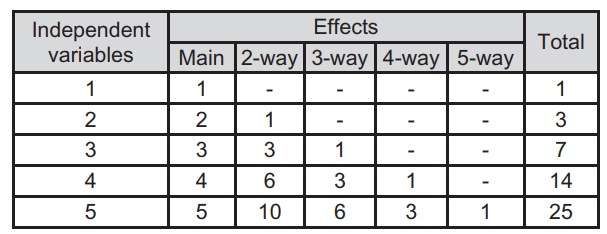
\includegraphics[width=0.5\linewidth]{effect}
		\caption{Source: Fg. 5.2 (Mackenzie)}
	\end{figure}
\end{frame}


%\subsection{Participants}
%
%\begin{frame}
%\frametitle{Participants}
%\begin{itemize}
%	\item Choose participants (1 ) that are members of the \textbf{same population} of people to who results are assumed to hold and (2) make sure you have \textbf{sufficient} participants
%	\item Way to determine how many participants: (1) see \textbf{commonality} in earlier work, (2) \textbf{power analysis} but in practice, it is rarely done because it requires knowing the variance in sample which is difficult
%	\item In average,\textbf{ 12-15} participants are sufficient.  One may also need to make sure the numbers of participants are sufficient such that all order of conditions are run equal
%	\item If participants are not sufficient, the downside is that \textbf{statistical test cannot be performed} since these test relied on reliable mean and variances
%	\item But as for usability evaluation (unlike factorial experiments), five participants are sufficient to expose 80 percent of usability problems
%\end{itemize}
%\end{frame}

%\begin{frame}
%	\frametitle{Reminders} % Table of contents slide, comment this block out to remove it
%	\begin{itemize}
%		\footnotesize
%		\item  \textbf{HW14 - 16} due Friday 28 Feb: this will provide a better understanding of how to design experiments
%		\item \textbf{First proposal draft} - INTRODUCTION AND RELATED WORK SECTION - use SIGCHI format (hard copy in class) - how long should it be?
%		\end{itemize}
%\end{frame}

%\begin{frame}
%	\frametitle{Reminders} % Table of contents slide, comment this block out to remove it
%	\begin{itemize}
%		\footnotesize
%		\item \textbf{Error bars} are important when plotting bar charts as it allows us to visually inspect the variability.  
%		\item To analyze the difference between correct and incorrect one, use\textbf{ bar charts}, put the correct and incorrect as x-axis, and analyze their average time and error rates for y-axis
%		\item To analyze the difference between blocks (each block has multiple trials), use \textbf{bar charts} representing attempt 1, 2, 3 as x-axis, and analyze the average time and error rates.
%		\item How to analyze whether number of boxes affect time and error rates, how to do?
%		\item Use {histogram} to show distributions (not bar charts or line charts)
%		\item \textbf{Trials} means one attempt, group of attempts are called \textbf{Blocks}  
%		\item \textbf{Tables} are only needed for writing average values, you almost never write the whole tables of raw data in a paper.  
%		\item Be careful what you \textbf{claim}, e.g., some of you said fatigue or boredom, which you did not measure
%		\item Only \textbf{three questions} and not more.
%	\end{itemize}
%\end{frame}

%\subsection{Independent and Dependent Variables}
%
%\begin{frame}
%	\frametitle{Independent Variables}
%	\begin{itemize}
%		\item Let's first decide the independent variables
%		\item \textbf{Independent variables} (IV) are variables you \textbf{manipulate}.  IV is also called a \textit{factor}.  
%		\item In HCI, \textbf{independent variables mostly are nominal}, such as device, input method, feedback modality, selection technique, menu depth, button layout, and so on
%		\item IV is usually manipulated across multiple \textbf{levels}  (also called test conditions)
%		\item When picking a IV, make sure you also consider different \textbf{sub-circumstances} (For text entry, one may text while \textit{sitting}, \textit{standing}, \textit{walking}).  In this way, your work will have two independent variables - text entry method and stance
%	\end{itemize}
%\end{frame}

%\begin{frame}
%	\frametitle{Independent Variables}
%	\begin{itemize}
%		\item It may be reasonable to have more than one IV, but once there are too many IV, it becomes \textbf{impossible to interpret}.  For example, a design with one IV has \textit{main effect} but no \textit{interaction effect}.  Two IV has two \textit{main effects} and one \textit{interaction effect}.  Three IVs - there will be seven effects!  \textbf{The recommended is usually two to three IVs, not too simple or too complicated.  Four or above is highly not recommended.}
%	\end{itemize}
%	\begin{figure}
%		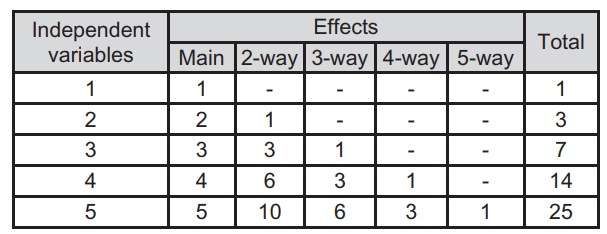
\includegraphics[width=0.7\linewidth]{effect}
%		\caption{Source: Fg. 5.2 (Mackenzie)}
%	\end{figure}
%\end{frame}

\subsection{Dependent Variable}

\begin{frame}
\frametitle{Dependent Variables}
Dependent variable (DV) is \textbf{what you measure} - they \textbf{depend} on the factors.  So what's our DV?
\end{frame}

\begin{frame}
\frametitle{Dependent Variables}
Dependent variable (DV) is \textbf{what you measure} - they \textbf{depend} on the factors.  So what's our DV?
\begin{itemize}
	\item For our case study:
	\begin{itemize}
		\item \textbf{Speed}: measured as completion time
		\item \textbf{Accuracy}: measured as error rate
		\item \textbf{Learning}: measured speed and accuracy improvements change over time
	\end{itemize}
	\item Good DVs are usually \textbf{numbers in continuous scale}
	\item Recommended to have \textbf{2-4 DVs}.  Why not too little or too much?
\end{itemize}
\end{frame}

\begin{frame}
	\frametitle{Dependent Variables}
	\begin{itemize}
		\item In HCI, the most common DV is \textbf{speed} (reported in task completion time) and \textbf{accuracy} (reported in error rate)
		\item Others include preparation time, action time, throughput, gaze shifts, mouse-to-keyboard hand transitions, preses of BACKSPACE, target re-entries, retries, key actions, gaze shifts
		\item Also some creative: count of negative facial expressions, number of times users shift their gaze from on-screen keyboard to the typed text.
		\item When reporting, it is important to see the \textbf{common units used in earlier work}, so your work can be compared 
%		\item \textbf{Dependent variable is typically a ratio-scale} such as task-completion time, error rate, number of button clicks, scrolling events, gaze shifts, etc.
	\end{itemize}
\end{frame}


%
%\begin{frame}
%	\frametitle{Dependent Variables}
%	\begin{figure}
%		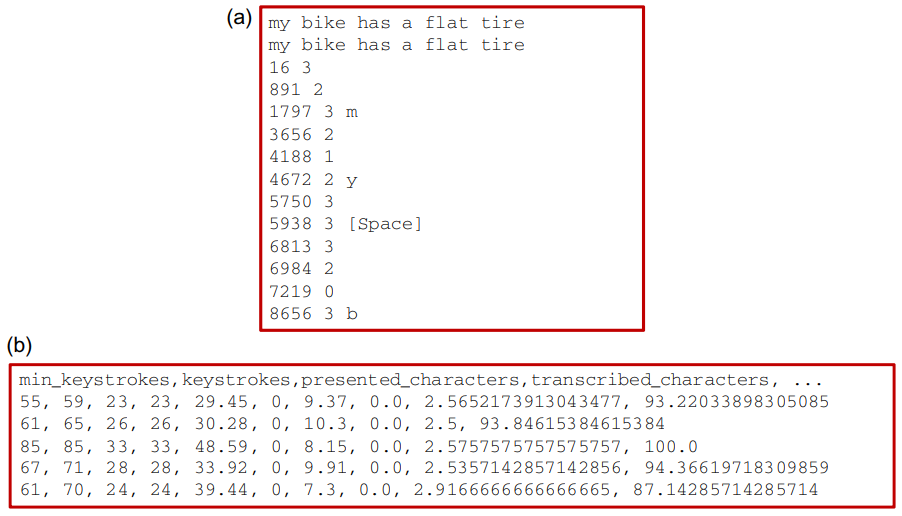
\includegraphics[width=0.9\linewidth]{logs}
%		\caption{Source: Fg. 5.3 (Mackenzie).  Naming logs for easier retrieval.  Name the file TextInputHuffman-P01-D99-B06-S01.  Participant 1, Device (D99), Block (B1), Session (S1)}
%	\end{figure}
%\end{frame}
%
%\begin{frame}
%\frametitle{Dependent Variables}
%\begin{itemize}
%	\item The starting point of research is observe, so how to we observe in HCI?
%	\begin{itemize}
%		\item \textbf{Log} of users' action - need to make sure we can reproduce what users did (measured in ms)
%		\item Important \textbf{events} include key presses, mouse movement, selections, finger touches, finger swipes, and associated timestamps
%		\item When users' action cannot be recorded by computers, \textbf{video recordings} are helpful to record such behaviors
%	\end{itemize}
%\end{itemize}
%\end{frame}

\subsection{Other Variables}

\begin{frame}
	\frametitle{Other Variables}
	\begin{itemize}
		\item Other variables are \textbf{noise} variables that we want to either control (\textbf{Control} Variables),  allow to vary (\textbf{Random} Variables), or do our best to mitigate (\textbf{Confounding} Variables).  
		\item Note that a variable can be either Control, Random or Confounding, depends on how you look at them.
	\end{itemize}
\end{frame}

\begin{frame}
	\frametitle{Control Variables}
	\begin{itemize}
		\item  \textbf{Control} variables are factors the might influence IV such as room lighting, room temperature, background noise, selection of mouse.  Researchers ought to \textbf{control} these variables so they are the same across during the experiment for all participants.
		\item So our study?
	\end{itemize}
\end{frame}

\begin{frame}
	\frametitle{Control Variables}
	\begin{itemize}
		\item  \textbf{Control} variables are factors the might influence IV such as room lighting, room temperature, background noise, selection of mouse.  Researchers ought to \textbf{control} these variables so they are the same across during the experiment for all participants.
		\item So our study?
	\end{itemize}
	For our case study:
	\begin{itemize}
		\item \textbf{Control} variables for our experiment are computers, mouse, monitor, experimental time, environment, instructions, etc. which \textbf{should be} controlled as constant across participants
	\end{itemize}
\end{frame}

\begin{frame}
	\frametitle{Random Variables}
	\begin{itemize}
		\item \textbf{Random} variables are variables that researchers may allow to vary such as age or gender of participants, personality.  Usually a well-design experiment can mitigate these effects
		\item Our study?
	\end{itemize}
\end{frame}

\begin{frame}
	\frametitle{Random Variables}
	\begin{itemize}
		\item \textbf{Random} variables are variables that researchers may allow to vary such as age or gender of participants, personality.  Usually a well-design experiment can mitigate these effects
		\item Our study?
	\end{itemize}
	For our case study:
	\begin{itemize}
		\item \textbf{Random} variables are participants' age, gender, background which we cannot control, but a well-designed experiment will help.  At least, we need to record these info.
	\end{itemize}
\end{frame}

\begin{frame}
	\frametitle{Confounding Variables}
	\begin{itemize}
		\item \textbf{Confounding} variables are possible noise variables that can contaminate our experiment.
		\item What's our possible confounding vars?
	\end{itemize}
\end{frame}

\begin{frame}
	\frametitle{Confounding Variables}
	\begin{itemize}
		\item \textbf{Confounding} variables are possible noise variables that can contaminate our experiment.
		\item What's our possible confounding vars?
	\end{itemize}
	For our case study:
	\begin{itemize}
		\item \textbf{Confounding} variables are \textbf{learning effect},  \textbf{individual differences}, and \textbf{implementation of pie menu and linear menus}
	\end{itemize}
\end{frame}

%\begin{frame}
%\begin{center} 
%\usebeamerfont*{frametitle} \usebeamercolor[fg]{frametitle}  5-mins break 
%\end{center}
%\end{frame}

%
%\begin{frame}
%	\frametitle{Confounding Variables}
%	\begin{columns}[c] % The "c" option specifies centered vertical alignment while the "t" option is used for top vertical alignment
%		
%		\column{.5\textwidth} % Left column and width
%			\begin{figure}
%			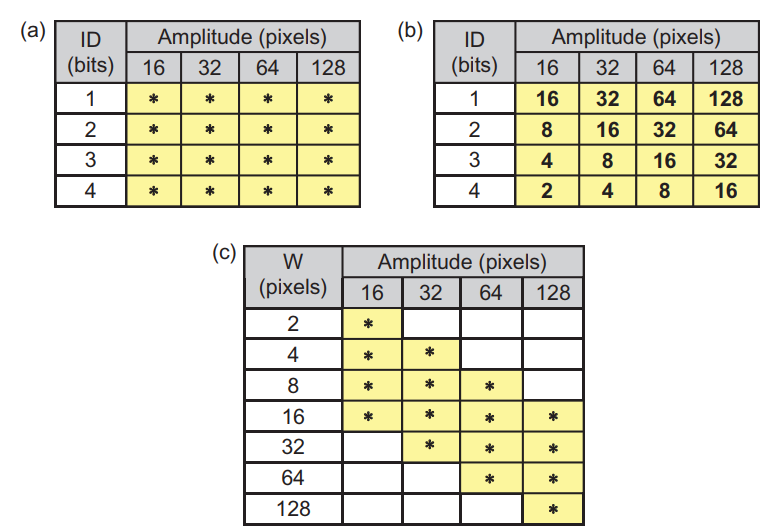
\includegraphics[width=1\linewidth]{fitts}
%			\caption{Source: Fg. 5.5 (Mackenzie).}
%		\end{figure}
%		
%		\column{.5\textwidth} % Right column and width
%		\footnotesize
%		\begin{itemize}
%			\item Confounding variables are sometime found in \textbf{Fitts' law experiments}
%			\item Most Fitts’ law experiments use a target selection task with movement amplitude (A) and Index of difficulty (ID) as independent variables (ID = ${\log_2 (2A/W)} $) 
%			\item If A has levels 4, 8, 16, 32cm, and ID with 1, 2, 3, 4.  It will yield 16 test conditions.  
%			\item As ID increases, W decreases.  Target width becomes a confounding variable.    If the experiment found a main effect of ID, is the effect due to ID or to W?
%		\end{itemize}
%	\end{columns}
%
%\end{frame}
%
%\begin{frame}
%\frametitle{Confounding Variables}
%\begin{itemize}
%	\item \textbf{Casual} relationship describes a \textit{cause-and-effect} relationship between IV and DV
%	\item Researchers have to beware for \textbf{circumstantial} relationship, that is, relationship \textit{by circumstances or environment}
%\end{itemize}
%	\begin{figure}
%	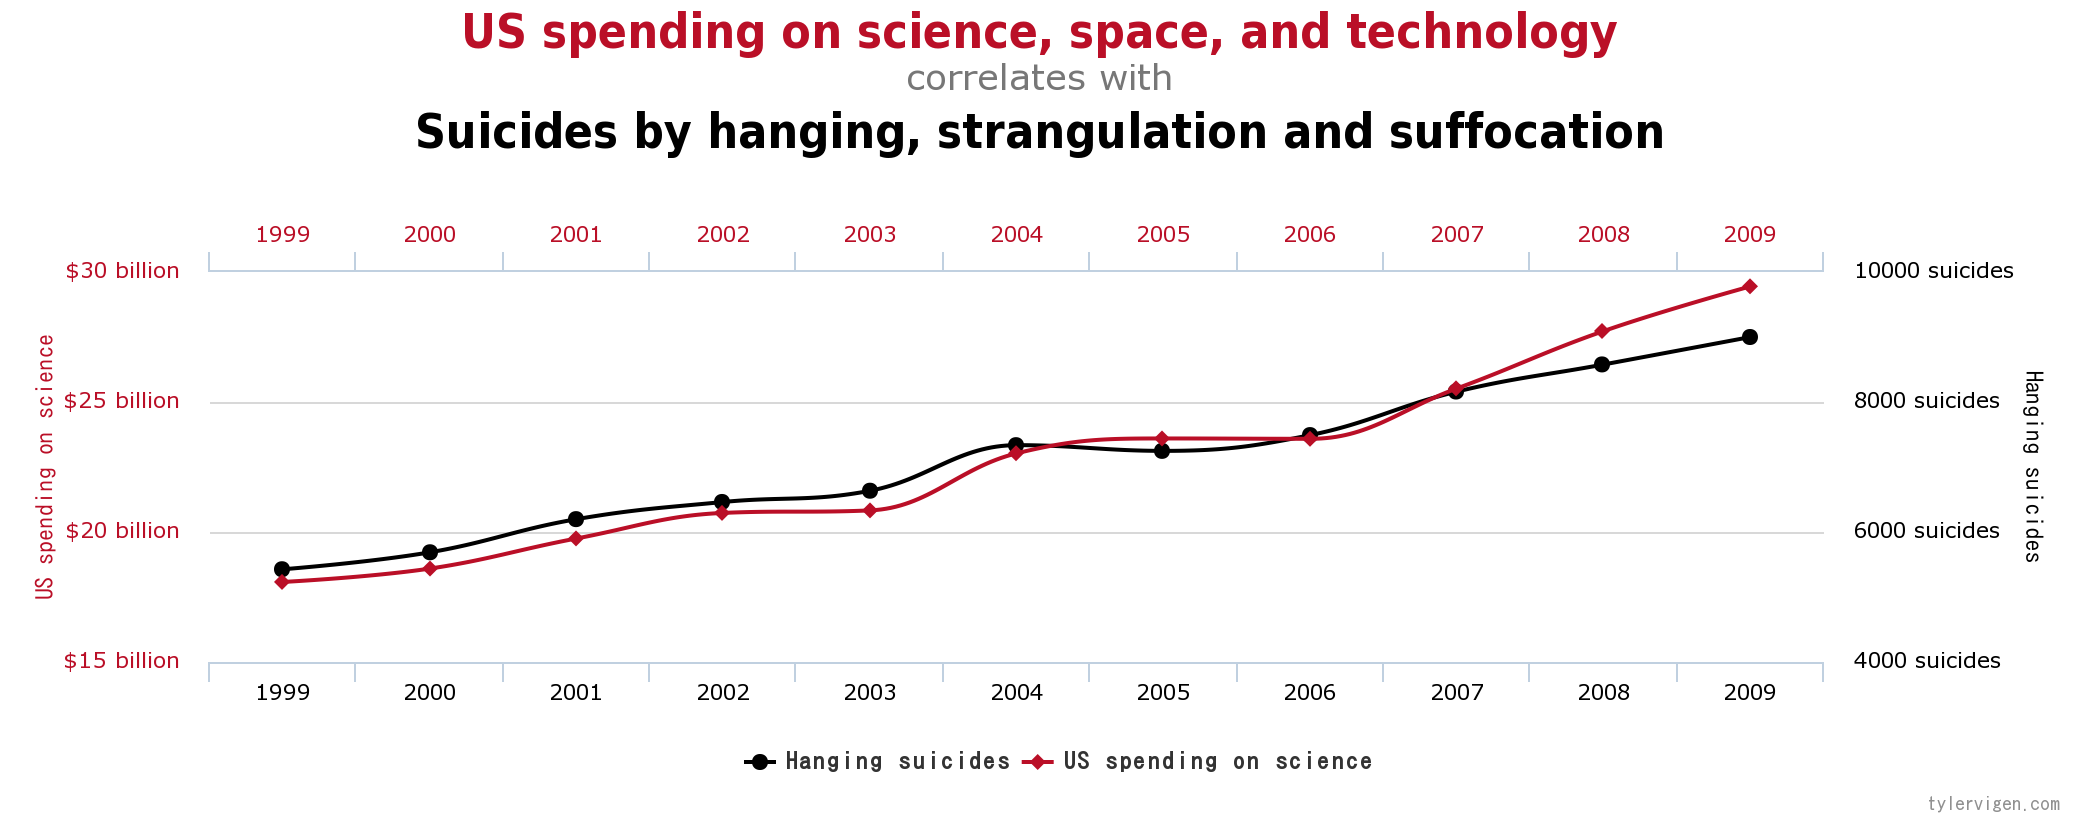
\includegraphics[width=1\linewidth]{causeeffect}
%	\caption{Source: Spurious Correlation by Tyler Nglen.}
%\end{figure}
%\end{frame}
%
%\begin{frame}
%\frametitle{Confounding Variables}
%\begin{itemize}
%\item Another example: we found 15 users who uses T9, and 15 users who uses QWERTY.  Their speed was measured.  We found that QWERTY was faster!  But this is a circumstantial relationship because the differences may due to individual differences.
%\item To avoid circumstantial relationship,\textbf{ controlled experiment }is required.  However, cause-and-effect conclusions can not be done with \textit{naturally occurring attribute} such as gender, personality, handedness, and so.  It is difficult to know whether the experimental effect was due to these independent variables or to the confounding variables
%\end{itemize}
%\end{frame}


\subsection{Within- and between-subjects}


\begin{frame}
\frametitle{Within- and between-subjects}
\begin{itemize}
	\item Should we test all conditions with all participants?
	\item Or each condition with each group of participants?
\end{itemize}
\end{frame}

\begin{frame}
\frametitle{Within- and between-subjects}
\begin{itemize}
	\item \textbf{Within-subjects} is when each participant is tested on each levels.  Is also called \textit{repeated measures}
	\item \textbf{Between-subjects} is when each participant is tested on only one level.  
\end{itemize}
\begin{figure}
	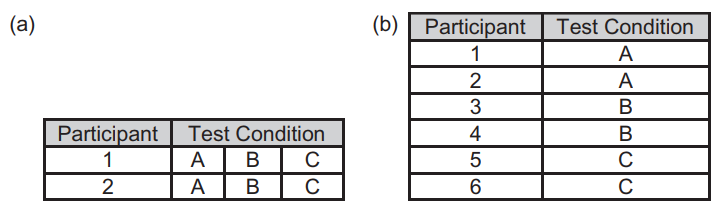
\includegraphics[width=1\linewidth]{within}
	\caption{Source: Fg. 5.6 (Mackenzie).  a) Within-subject, b) Between subject}
\end{figure}
\end{frame}

\begin{frame}
\frametitle{Within- and between-subjects}
\begin{itemize}
\item \textbf{Within-subjects} uses \textbf{less} participants, prone to \textbf{practice effect} and thus require more \textbf{testing}.  Usually preferred.
\item \textbf{Between-subjects} uses \textbf{more} participants, prone to \textbf{effect of individual differences} and thus require effort to \textbf{balance} all groups.  However, certain experiments require between-subject such as drug experiment or gender experiment  
\item \textbf{Mixed-design} uses both within-subject and between-subject in one design.  For example, the experiment has two factors: block is within-subjects with perhaps 10 levels (block 1, block 2...) and handedness is between-subjects with two levels (left, right)
\end{itemize}
\end{frame}

\begin{frame}
\frametitle{Within- and between-subjects}
In our study, within-subject is the clear choice.   Choosing between-subject will 	\textbf{require lots of participants} in order to balance out the effect of individual differences.  The more factors (subsequently the conditions), the more participants we are required which is costly.  On the other hand, within-subject is prone to \textbf{practice/learning effect} which can be easily fixed by administering \textbf{block design.}
\end{frame}

%\begin{frame}
%	\frametitle{When to use between-subject?}
%	\begin{itemize}
%%		\item Counterbalancing mitigates \textbf{practice effect / learning effect}.  However, this is only true when we assume that different order (e.g., A first then B and B first then A) has the same effect
%%		\item If the above assumption is incorrect, there is a \textbf{group effect} and is typically due to \textbf{asymmetric skill transfer}, i.e., there is certain skill transfer from one task to another
%		\item Consider an IV with two levels (A:keyboard, and B:keyboard with word prediction).  Participants who do A then B were found to perform better than B then A, because participants are allowed to learn the easier method first in A (Koester and Levine, 1994a), this is called \textbf{skill transfer}
%		\item In this kind of case, it is recommended to use \textbf{between-subject design}
%		\item Similar phenomenon can be observed in education or drug experiment.
%	\end{itemize}
%\end{frame}


\subsection{Order Effects}

\begin{frame}
\frametitle{Order Effects}
Do you think the order of IV conditions matters?
\vspace{20pt}

If yes, how we should best order it?
\end{frame}

\begin{frame}
\frametitle{Order Effects - Latin Square}
\begin{itemize}
\item Order of conditions may affect the results, e.g., \textbf{fatigue}, \textbf{learning effects}.  Thus it is necessary to \textit{counterbalance} the order of conditions across participants
\item \textbf{Latin Square} is a common method for counterbalancing.  %For example, if there are 12 participants and there are two test conditions,  half of them does condition A first, while rest of them does condition B first.
%\item %For more conditions, the idea is to make sure the set of order of conditions should be \textbf{equal}.  Also it is important to have \textbf{sufficient participants} to fill in these sets   
\end{itemize}
\begin{figure}
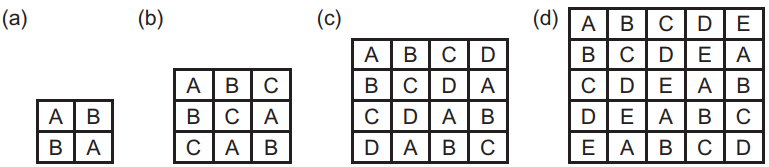
\includegraphics[width=0.8\linewidth]{latin}
\caption{Source: Fg. 5.7 (Mackenzie).  Here A, B, C, etc. represent conditions or combined conditions.}
\end{figure}
\end{frame}

\begin{frame}
\frametitle{Order Effects - Balanced Latin Square}
\begin{itemize}
%\footnotesize
\item A deficiency in Latin squares of order 3 and higher is that conditions precede and follow other conditions an \textbf{unequal} number of times. In the 4 $ x $ 4 Latin square, for example, B follows A three times, but A follows B only once 
\item \textbf{Balanced Latin-square} addresses this. The top row has the sequence A, B, \textit{n}, C, \textit{n-1}, D, \textit{n-2}, etc. For following rows, simply add 1
%\item For balanced latin-square, number of participants depend on the \textbf{number of levels}, e.g., if a factor has three levels, then the experiment requires multiple-of-3 participants (3, 6, 9, 12, etc.)
\end{itemize}
\begin{figure}
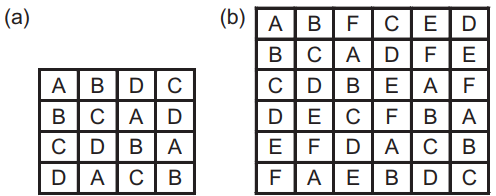
\includegraphics[width=0.5\linewidth]{balanced}
\caption{Source: Fg. 5.8 (Mackenzie).}
\end{figure}
\end{frame}

%\begin{frame}
%\frametitle{Order Effects - Latin Square}
%\begin{itemize}
%\item The one drawback of balanced Latin squares is that it only works for \textbf{even} number of test conditions
%\item As an example of this drawback, imagine an experiment with one IV with \textbf{three} levels (A, B, C), where each level depicts a different editing method (e.g., search and replace)
%\item Each participant does the task \textbf{five} times with each editing method, then does the same with other methods
%\item Order of levels are counterbalanced, where group 1 (participant 1, 2, 3, 4) follows \textbf{ABC}, group 2 follows \textbf{BCA}, and group 3 follows \textbf{CAB}
%\item This result is imbalanced because B follows A twice but A follows B only once
%\end{itemize}
%\end{frame}

%\begin{frame}
%\frametitle{Order Effects - Balanced Latin Square}
%\begin{figure}
%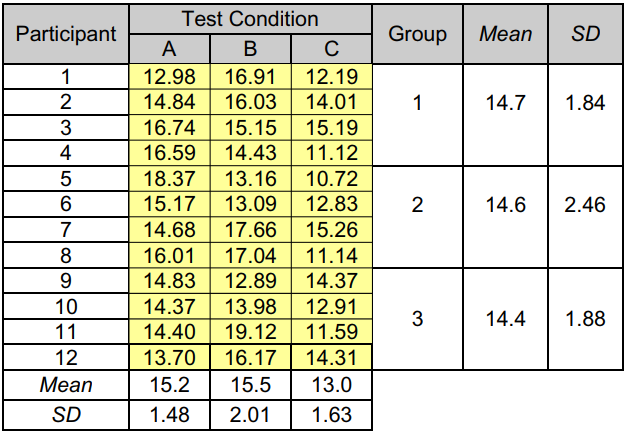
\includegraphics[width=0.9\linewidth]{balanced2}
%\caption{Source: Fg. 5.9 (Mackenzie).}
%\end{figure}
%\end{frame}

\begin{frame}
\frametitle{Order Effects - Full Latin Square}
\begin{itemize}
\item The one drawback of balanced Latin squares is that it only works for \textbf{even} number of test conditions
\item One may draw out all possible combinations (n!) (\textbf{full-counter balancing}) but would require more participants (here we could recruit 18 participants, each set with 3 participants).  %Another way is to use \textbf{Latin square} where each condition appears in each position equally - ABC, BCA, CAB
\end{itemize}
\begin{figure}
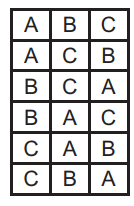
\includegraphics[width=0.2\linewidth]{full}
\caption{Source: Fg. 5.11 (Mackenzie).}
\end{figure}
\end{frame}

\begin{frame}
\frametitle{Order Effects - Randomization}
\begin{itemize}
\item Another way to address this imbalance is to simply \textbf{randomize} the order of conditions.  This is suitable when the task is \textbf{very brief}, there are many \textbf{repetitions} of the task, and there are \textbf{many test conditions}.  %For example, if an experiment has three factors each with multiple levels, it make sense to randomize the order
\item Last, it is recommended to look at \textbf{earlier works}, to see the common acceptable counterbalancing method  %(usually Latin square is sufficient but again, consult with papers related to your topic)
\end{itemize}
\end{frame}

\begin{frame}
\frametitle{Order Effects - Sequential}
\begin{itemize}
\item Last way to address this imbalance is to use \textbf{sequential} order of conditions.  This is suitable when the conditions you compared is of \textbf{increasing difficulty} by nature.   For example, if you have two condition of a small and big width, it might be okay to always do small before big width since there is \textbf{no learning effect} anyway.  %For example, if an experiment has three factors each with multiple levels, it make sense to randomize the order
\item Sequential is all about how you perceive the task whether it's an increasing difficulty task.  I recommended to use this only if you are very sure.  %(usually Latin square is sufficient but again, consult with papers related to your topic)
\end{itemize}
\end{frame}

\begin{frame}
	\frametitle{Order Effects}
	How about our study?
\end{frame}

\begin{frame}
	\footnotesize
	\frametitle{Order Effects}
	\begin{itemize}
		\item In our case, we have four IVs - menu type (MT) (2), breadth (B) (3), depth (D) (3), and usage (U) (2)
		\item The key here is to choose a reasonable order scheme that \textbf{minimize number of participants}, while reasonably mitigating learning effect.
		\item Since we have even number of conditions (2 x 3 x 3 x 2 = 36),  let's say we do \textbf{Balanced Latin Square},  we need a multiple of 36 participants,  which is a lot!
		\item Can we further minimize participants.?  Since \textbf{menu type} is our main factor, we don't want to compromise.  \textbf{Usage} is only two level,  so trying to do anything won't change much.   \textbf{Breadth} and \textbf{Width} worth 9 conditions - since this is a lot, we can change to \textbf{Randomized} scheme or even \textbf{Sequential} scheme (since the complexity increases accordingly)
%		\item \textbf{Menu type} - full counter-balanced - is only two level %so it is quite easy
%		\item \textbf{Usage} - full counter-balanced
%		\item \textbf{Breadth and width} - randomization or sequential
		%\item What we can do is simply performing sequential orders for breadth and depth.  This is doable when the difference is something of particular interest, since the differences are too obvious.Another way is to perform a randomize orders for breadth and width which is also fair.   
		\item Thus, we will have four conditions - MT1U1, MT1U2, MT2U1, and MT2U2.  We will denote them as A, B, C, D.   We can use balanced latin square which will give four sets: {ABDC, BCAD, CDBA, DACB}.  Thus our number of participants will be multiples of 4;  16 and 20 are good numbers.
	\end{itemize}
\end{frame}

\subsection{Task and Procedure}

\begin{frame}
	\frametitle{Task and Procedure}
	\begin{itemize}
%		\item Two objectives in designing a good task: \textit{represent} and \textit{discriminate}
%		\item \textbf{Represent}:  task that represent actual usage, to improve external validity
%		\item \textbf{Discriminate}: discriminate test conditions to make sure any effects found is due to differences in test conditions, to improve internal validity
		\item It is highly recommended to use the \textbf{same task} (or with slight variations) as past work, so to promote comparison and advancement of the field.  Also, they have already been well thought out.
		\item \textbf{Don't design your own procedure}, unless you have worked in the field for at least many years!
%		\item It is nothing wrong to use \textbf{exact same task} (with slight variations like conditions) as earlier work, in fact, it is recommended within the research society to promote comparison and advancement of the field
	\end{itemize}
\end{frame}

\begin{frame}
\frametitle{Task and Procedure}
\begin{itemize}
%	\item One specific challenge we need to tackle:
%	\begin{itemize}
		\item What if user makes mistake?
		\begin{itemize}
			\item use \textbf{trials}
		\end{itemize}
		\item What if we want to monitor their learning rate 
		\begin{itemize}
			\item use \textbf{blocks} - a repeated section of an experiment that consists of multiple trials in randomized orders.
			 \item use \textbf{session} - which is simply composed of multiple blocks
		\end{itemize}				
	\item So how many trials and blocks?  How about breaks?
	\begin{itemize}
		\item More blocks and more breaktime are always desirable but based on \textbf{experimental time}.   Why? \textbf{Reasonable duration is at max 1 hour.}
	\end{itemize}
\end{itemize}
\begin{figure}
		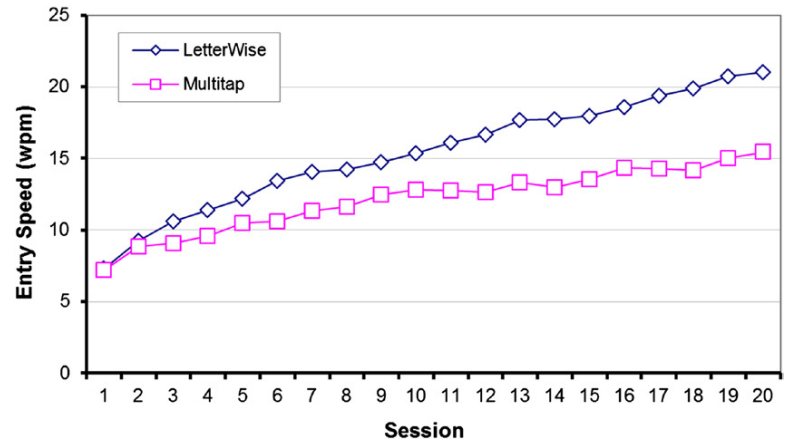
\includegraphics[width=0.3\linewidth]{long}
		
		\caption{Source: Fg. 5.16 (Mackenzie).  Two text-entry method were tested over 20 sessions; each session involved 30 minutes of text-entry.}
	\end{figure}
\end{frame}

\begin{frame}
\frametitle{Task and Procedure}
For our case study:
\begin{columns}[c] % The "c" option specifies centered vertical alignment while the "t" option is used for top vertical alignment
	
	\column{.6\textwidth} % Left column and width
	\begin{figure}
		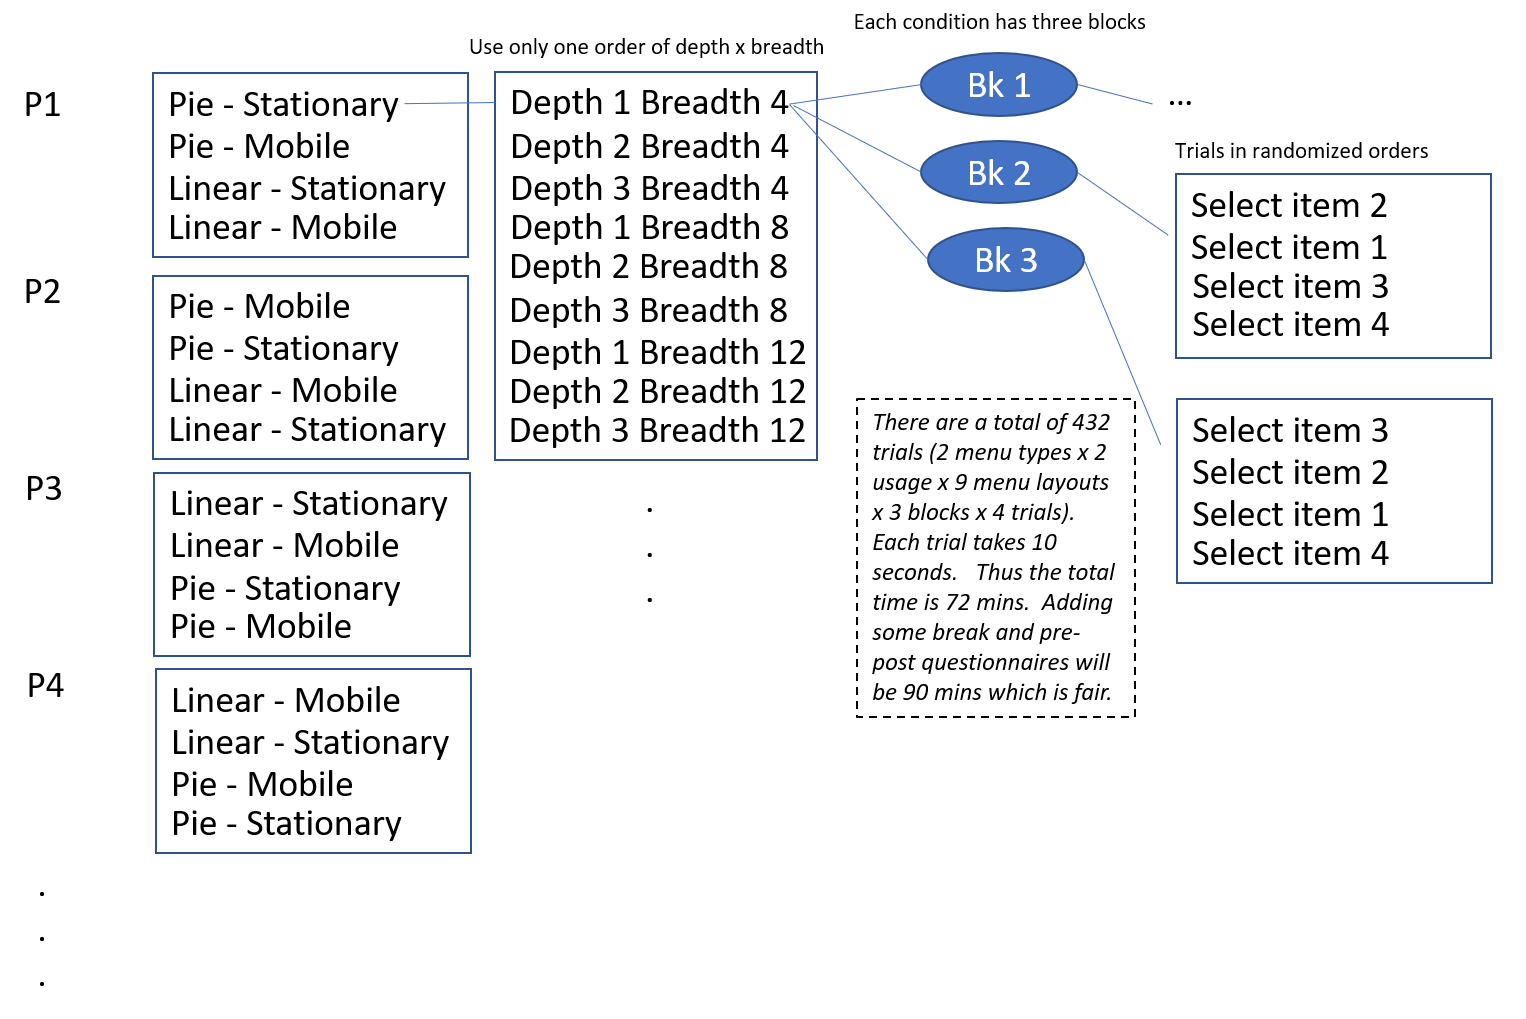
\includegraphics[width=1\linewidth]{design}
		\caption{Possible experimental design}
	\end{figure}
	
	\column{.4\textwidth} % Right column and width
	\vspace{-20pt}
	\footnotesize
	\begin{itemize}
		\item \textbf{Trials}: 4 trials where each trial select certain menu item as fast and as accurate as possible
		\item \textbf{Blocks}: 3 blocks consists of multiple trials in randomized orders that repeated for each condition 
		\item \textbf{Time}: 2 \textbf{input} methods $x$ 2 \textbf{postures} $x$ 3 \textbf{depth} $x$ 3 \textbf{breadth} $x$ 3 \textbf{blocks} $x$ 4 \textbf{trials} $x$ 2s = 864s = 14.4 mins + 35 \textbf{breaks} $x$ 1 min  = 49.4 mins
		\item How did I determine the break time or blocks?
	\end{itemize}
\end{columns}

\end{frame}

\begin{frame}
	\frametitle{Task and Procedure: Example}
	\begin{itemize}
		\item Procedure:
		\begin{enumerate}
			\item Consent form and pre-experiment questionnaires
			\item Instructions
			\begin{itemize}
				\item First, a menu item will be shown on display to indicate target
				\item Second, user presses space-bar button to indicate "start"
				\item Third, user select the target menu item as fast and as accurate as possible
				\item Fourth, a moment of pause before going back to first
			\end{itemize}
			\item Practice trials
			\item Main experiment with breaks
			\item Post-experiment questionnaires
		\end{enumerate}
	\end{itemize}
\end{frame}

%\begin{frame}
%\begin{center} 
%\usebeamerfont*{frametitle} \usebeamercolor[fg]{frametitle}  5-mins break 
%\end{center}
%\end{frame}


\subsection{Questionnaire Design}

\begin{frame}
	\frametitle{Questionnaire Design}
	\begin{itemize}
		\item Two purposes: (1) gather information on \textbf{demographics} (age, gender, etc.) and experience with related technology, (2) gather \textbf{opinions} at the \textbf{end of experiment}
	\end{itemize}
		\centering
		\begin{figure}
			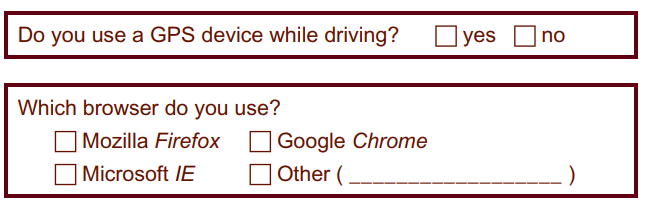
\includegraphics[width=0.5\linewidth]{gps}
		\end{figure}
		\begin{figure}
			
\includegraphics[width=0.5\linewidth]{browser}
		\end{figure}
		\begin{figure}
			
\includegraphics[width=0.5\linewidth]{age}
		\end{figure}
		\begin{figure}
			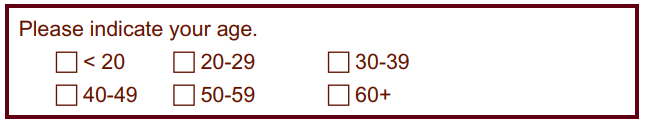
\includegraphics[width=0.5\linewidth]{age2}
		\end{figure}
\end{frame}

\begin{frame}
	\frametitle{Questionnaire Design}
	\begin{itemize}
		\item \textbf{Avoid creating your own questionnaires}.  Making questionnaires requires some statistical proof so it's not easy.   Follow the proven ones.
		\item Check with your past work what questionnaires they use.  \textbf{ Follow them.}
	\end{itemize}
\end{frame}

%\begin{frame}
%	\frametitle{Questionnaire Design}
%	\begin{itemize}
%		\item One common questionnaire to use at the end of experiment is NASA-TLX (task load index), which assesses perceived workload on six subscales: mental demand, physical demand, temporal demand, performance, effort, and frustration.  
%	\end{itemize}
%	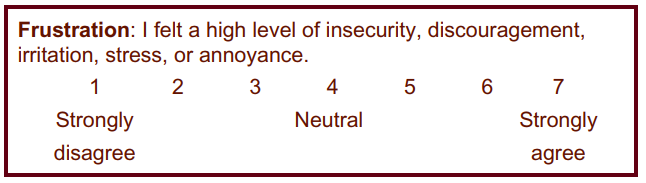
\includegraphics[width=1\linewidth]{tlx}
%\end{frame}
%
%\begin{frame}
%	\frametitle{Questionnaire Design}
%	\begin{itemize}
%		\item The ISO 9241-9 standard for non-keyboard input devices includes a questionnaire with 12 items to assess the comfort and fatigue experienced by participants (ISO 2000).  The items are similar to those in the NASA-TLX but are generally directed to interaction with devices such as mice, joysticks, or eye trackers.
%	\end{itemize}
%	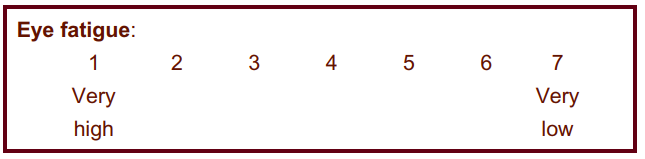
\includegraphics[width=1\linewidth]{iso}
%\end{frame}

\subsection{Experiment Validity}

\begin{frame}
\frametitle{Validity Analysis}
\begin{itemize}
\item Consider an experiment that compares \textbf{two gestures technique for TV}, which experimental design?
\begin{enumerate}
\item  Tested in a real-world environment -  \textbf{large sofa} with a \textbf{large TV}.  They can watch anything.  They can also eat.  No instructions given.
\item Tested in a \textbf{controlled environment} - more-controlled - task, procedure, IV, DV.
\end{enumerate}
\end{itemize}
\end{frame}

\begin{frame}
\frametitle{Internal and External Validity}
\begin{figure}

\includegraphics[width=0.9\linewidth]{internalexternal2}
\caption{Source: Fg. 4.9 (Mackenzie)}
\end{figure}
\end{frame}

%\begin{frame}
%\frametitle{Internal and External Validity}
%\begin{figure}
%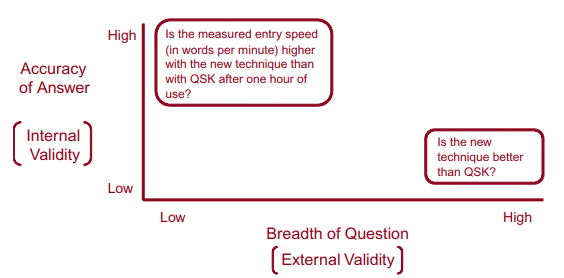
\includegraphics[width=0.9\linewidth]{internalexternal}
%\caption{Source: Fg. 4.8 (Mackenzie)}
%\end{figure}
%\end{frame}

\begin{frame}
\frametitle{Internal Validity}
\begin{itemize}
	\item \textbf{Internal Validity} is the extent to which an effect observed is due to test conditions
	\begin{itemize}
		\item When you are comparing two conditions, did you make sure everything else is \textbf{equal} except what you are manipulating?
		\item Did you correctly \textbf{order} the experimental conditions?
		\item Did you assign users to different groups in a \textbf{randomized} way?
		\item Did you take care \textbf{learning effects} by applying appropriate training before the experiment or applying block design?
%		\item Basically, any \textbf{potential noise} lowers internal validity
	\end{itemize}
\end{itemize}
\end{frame}

\begin{frame}
\frametitle{External Validity}
\begin{itemize}
\item \textbf{External Validity} is your result \textbf{generalized} across people and contexts
\begin{itemize}
	\item \textbf{Representative} participant? %of the world?
	\item \textbf{Representative} task? %of the world?
	\item \textbf{Representative} tool? %of the world?
	%\item Basically, if your result is specific to your experiment, it lowers external validity
\end{itemize}
\end{itemize}
\end{frame}


%\begin{frame}
%\frametitle{Text-Entry: Validity Analysis}
%\begin{itemize}
%\item  Consider an experiment comparing two methods of text entry, 
%\item  To improve \textbf{external validity}, participants are instructed to enter whatever text they think of. The text may include punctuation symbols and uppercase and lowercase characters, and participants can edit the text and correct errors as they go
%\item However, \textbf{internal validity} is compromised because noise behaviors are introduced such as pondering (What should I enter next?) and fiddling with commands (How do I move the cursor back and
%make a correction?). Furthermore, since participants generate the text, errors are difficult to record since there is no ``source text" with which to compare the entered text
%\end{itemize}
%\end{frame}

\begin{frame}
\frametitle{Internal vs. External Validity}
\begin{itemize}
\item The idea is that in research, \textbf{internal validity} cannot be compromised.  As for external validity, researchers have to do their best in a way that their work achieve the \textbf{highest external validity possible} and also \textbf{acknowledge the limitation} in their work.
\end{itemize}
\end{frame}

\begin{frame}
\frametitle{Construct Validity}
\begin{itemize}
\item is the extent to which you are \textbf{measuring things} based on what you claim
\begin{itemize}
\item Measuring \textbf{happiness} but uses only interview or user preference%  or measuring text-entry performance with only speed but not errors
\item Measuring \textbf{typing performance }but ignore that people can type while walking %while they are walking or sitting or standing
\item Talking about \textbf{habit} formation but collect data using only five days experiment
\end{itemize}
\end{itemize}
\end{frame}

\subsection{Last Notes}

\begin{frame}
	\frametitle{Practical suggestions}
	\footnotesize
	\begin{itemize}
		\item \textbf{Reminders}:  RQ $\rightarrow$ Hypothesis $\rightarrow$ Design and Implementation $\rightarrow$ Experimental Design $\rightarrow$ statistical analysis
		\item Always do a \textbf{pilot study.}   It's almost 99\% that your first experimental design will always be imperfect.
		\item There are \textbf{NOT only one experimental design solution;  some decisions are arguable}.   Of course, there are also many obviously wrong design.
		\item Try not to make your own task or questionnaires.  \textbf{Follow papers}.   This will make your work comparable, and also valid.
		\item \textbf{One hour} is just approximate.  Some experiment is more tiring, so make sure your participants are fresh.   If needed, split the experiment into several studies.
		\item I didn't talk much about \textbf{iterative experiment}, which is about having no clear IV, but instead iteratively explore your solution with your users directly.   This is usually inefficient but only intended for people with no idea about their IV.  \textbf{If you cannot think about what is your IV or hypothesis, usually because you don't understand enough.}
	\end{itemize}		
\end{frame}

\begin{frame}
	\frametitle{Link to project}
	\begin{itemize}
		\item Any papers you read should be \textbf{experimental}, i.e., have clear IV and DV. 
		\item You can attempt on any topic you want, but it should compose of experimental components, i.e., you should have clear, specific \textbf{research question}, \textbf{hypotheses}, and \textbf{experimental design}. 
		\item Why Chaky emphasizes \textit{experimental} papers, but does not encourage reading \textit{exploratory} papers?
	\end{itemize}		
\end{frame}

\begin{frame}
\frametitle{What's next}
	\begin{itemize}
		\item Next coming week 3 workshops on experiment.   Read and try the workshops before coming to class.
	\end{itemize}
\end{frame}

%\subsection{Longitudinal Studies}
%
%\begin{frame}
%	\footnotesize
%	\frametitle{Longitudinal Studies}
%	\begin{itemize}
%		\item Sometimes, \textbf{acquisition of skills} or \textbf{improvement of performance} is of interest.  In this case, testing users over a prolonged period of time called \textit{longitudinal study} will be preferred
%		\item In a longitudinal study, \textbf{amount of practice} is an independent variable. A typical name is \textit{Session} with levels 1, 2, 3 and so on, where each session involves multiple trials (repetitions) of the task.  Sessions composed of multiple blocks.
%	\end{itemize}
%	\begin{figure}
%		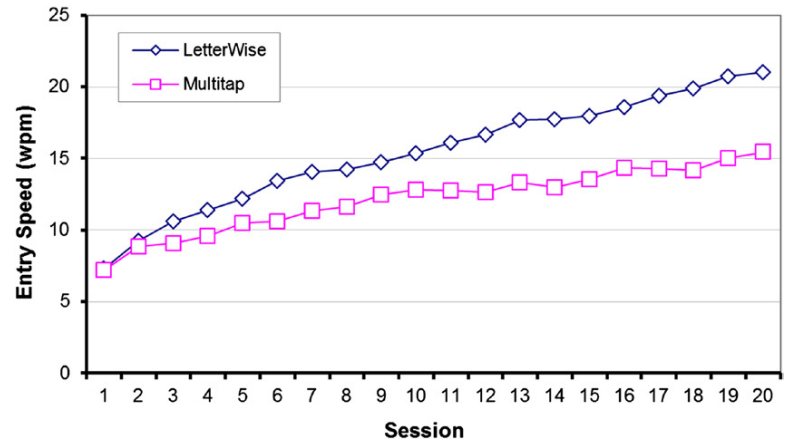
\includegraphics[width=0.4\linewidth]{long}
%		
%		\caption{Source: Fg. 5.16 (Mackenzie).  Two text-entry method were tested over 20 sessions; each session involved 30 minutes of text-entry}
%	\end{figure}
%\end{frame}
%
%\begin{frame}
%	\frametitle{Longitudinal Studies}
%	\begin{itemize}
%		\item In a longitudinal study, \textbf{crossover point} defines the point where the performance of one technique \textit{crossover} another technique as learning progresses
%		\item For example, in a comparison of QWERTY and Dvorak, Dvorak showed superior performance over QWERTY.  QWERTY remains because the cost is too high
%	\end{itemize}
%	\begin{figure}
%		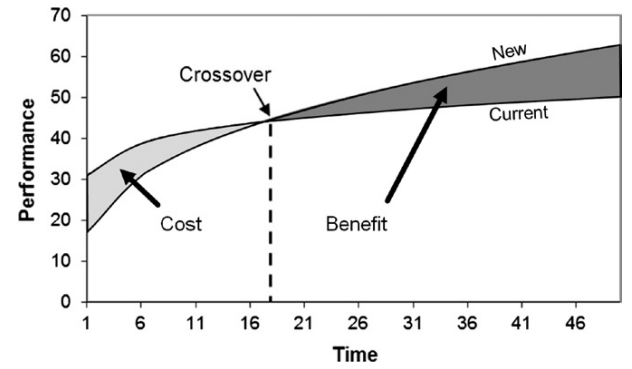
\includegraphics[width=0.6\linewidth]{crossover}
%		\caption{Source: Fg. 5.17 (Mackenzie).}
%	\end{figure}
%\end{frame}

%\subsection{Tips: Running the Experiment}
%
%\begin{frame}
%\frametitle{Ethics Approval}
%\begin{itemize}
%	\item Since HCI is about humans, researchers must respect the safety, welfare, and dignity of human participants
%	\item Human participants have the right to be informed of the followings:  purpose of the research, methodology, any risks or benefits
%	\item One can search for template for ethics approval
%\end{itemize}
%\end{frame}
%
%\begin{frame}
%	\frametitle{Running the Experiment}
%	\begin{itemize}
%		\item Always useful to have a \textbf{pilot test} with one or two participants
%		\item Important aspect of the experiment is the \textbf{instructions} given to participants; for most interaction tasks, the participant is expected to proceed quickly and accurately but comfortably
%		\item If participants ask for \textbf{clarification}, caution must be exercised; any additional explanation that might motivate a participant to act differently from other participants is to be avoided
%		\item Experimenter should portray himself or herself as \textbf{neutral}.  Participants should not feel under pressure.  Participants should also not feel too relaxed.
%	\end{itemize}
%\end{frame}

\section{Workshop}

\begin{frame}
	\frametitle{1st Workshop}
	\footnotesize
	\begin{block}{Task}	
	Given two baseline input methods: \textbf{QWERTY} and \textbf{T9}, and our proposed method: \textbf{Swiping Gestures} which we claim to be faster and more accurate.   Design an experiment discussing:
	\begin{itemize}
	\item Research question
	\item Hypotheses
	\item Independent variables
	\item Dependent variables
	\item Any possible confounding/random/control variables
	\item Within or Between subject design
	\item Task
	\item Order
	\item Total experimental time
	\end{itemize}
	\end{block}
\end{frame}

\begin{frame}
	\footnotesize
	\frametitle{Solution}
	\begin{itemize}
     \item \textbf{RQ} - How does swipe compared to QWERTY and T9 in different context, such as in different screen sizes where swipe may not have clear advantage?
     \item \textbf{Hypotheses}
     \begin{itemize}
     	\item H1:  Swipe outperform QWERTY and T9 in terms of speed in small screen size
     	\item H2:  In big screen size,  there is no significant difference between Swipe and the other methods.
     	\item H3:  For learning,  users should be able to learn Swipe and start to show a better performance than QWERTY and T9 after some blocks of trials.
     	\item H4:  Swipe may have lower accuracy, since it varies based on the capabilities of the word prediction.
     \end{itemize}
		\item \textbf{IV} - \textbf{input methods} - 3 levels (QWERTY, T9, SWIPE);  Let's say we have one more IV that is \textbf{Screen size} with 2 levels (Small and Large).  This becomes a 3 $x$ 2 factorial design with 6 conditions.
		\item \textbf{DV} - speed, accuracy, and learning over blocks
	\end{itemize}
\end{frame}

\begin{frame}
	\footnotesize
	\frametitle{Solution}
	\begin{itemize}
		\item\textbf{Control variables} - place, phone, key feedback, key font, etc.
		\item \textbf{Random variables} - past experience
		\item \textbf{Confounding variables} - implementation, task, order
		\item \textbf{Within-subject design} - learning can be mitigated
		\item \textbf{Task} -  representative number of occurrences of character (perhaps use some proven dataset like \url{http://www.yorku.ca/mack/PhraseSets.zip})
		\item \textbf{Order} - We counterbalance using balanced latin square thus we need at least a multiple of 6 participants.   12 or 18 are good number.
		\item \textbf{Total time} - 3 input methods $x$ 2 screen size $x$ 3 blocks $x$ 6 random phrases $x$ 28s = 3024s = 50 mins + 5 breaks $x$ 1 min = 55 mins
	\end{itemize}
\end{frame}

\begin{frame}
	\frametitle{2nd Workshop}
	\begin{block}{Task}	
	\footnotesize
	\begin{itemize}
	\item \textbf{Research Question}:Which body parts are suitable for wearable vibration feedback in walking navigation for blind people?
	\item \textbf{Independent variables}: body parts (ears, neck, wrist, hand, chest, waist, ankle, front foot, mirrored on both sides), postures (standing, normal walking, fast walking), stimulus durations (700ms, 1000ms, 1500ms, 2000ms)
	\item \textbf{Dependent variables}: Perceivability and subjective perferences
	\item \textbf{Design the rest of the experiment}, including hypotheses, the task and procedure, the place of experiment, the participants, the order effects, number of trials and blocks, and last, calculate the total time of the experiment
	\end{itemize}
	\end{block}
\end{frame}

\begin{frame}
	\frametitle{2nd Workshop Solution}
	\footnotesize
	\begin{itemize}
		\item \textbf{Hypothesis} could be something like \em{Upper body parts overall performed best}, \textit{Longer stimulus durations may be needed for lower body parts}, \em{Walking will generally require longer stimulus durations}
		\item Possible \textbf{design}: 16 body positions x 3 postures x 4 durations x 3 trials = 576 trials
		\item Since each \textbf{trial} takes around 1s (actually 1.3s)  with 2.5s in between, the total time is 3.5s x 576 - 2.5s = 2013.5s / 60 = 33.558 mins - this is fair amount of time when counting time for filling questionnaires
		\item The \textbf{order} of body positions and stimulus duration were randomized but each body position will receive exactly 3 trials for each stimulus duration.  After one posture is done, we swap to another posture.  The order of posture is done using Latin-square
		\item The \textbf{speed of walking} must be controlled across participants (1.25m/s).  The fast walking was using 4.5m/s
		\item \textbf{Participants} could be blind people or teenagers depending on the target audience.  15 should be nice numbers since it's the 3s multiple of the Latin-square
		\item \textbf{Place of environment} - could be another IV but would require another study
		\item After each posture, participants rated their perception of the vibration for each body position, with 1 - most difficult to perceive and 7 as easiest to perceive
		\item Devices could be any arduino vibrators like Lilypads
	\end{itemize}
\end{frame}

\begin{frame}
	\frametitle{3rd Workshop}
	\begin{block}{Task}	
	\begin{figure}
		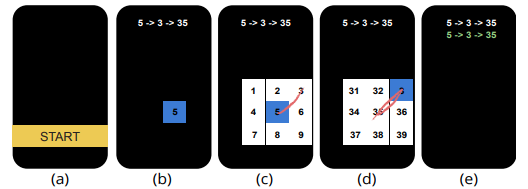
\includegraphics[width=0.5\linewidth]{gestures}
		\caption{Source: Zheng et al. CHI 2018}
	\end{figure}
	\vspace{-15pt}
	\footnotesize
	\begin{itemize}
		\item \textbf{Research Question}:We have proposed a gesture menu used in mobile phones - How does the newly proposed gesture menu compared to linear menu (baseline)?
		\item \textbf{Independent variables}: Input method (linear menu vs. gesture menu), Depth (1, 2, 3), Execution (guided, recall)
		\item \textbf{Dependent variables}: Time and error rates
		\item \textbf{Design the rest of the experiment}, including the task and procedure, the participants, the order effects, number of trials and blocks, and last, calculate the total time of the experiment
	\end{itemize}
	\end{block}
\end{frame}

\begin{frame}
	\frametitle{3rd Workshop Solution}
	\footnotesize
	\begin{itemize}
		\item \textbf{Depth} is one of the challenge.  In D1, there are 8 possible gestures, D2 - 64 gestures, D3 - 512 gestures.  To test all depths, it is possible to test completely D1 and 2 gestures, not but D3.  And due to time, we definitely cannot test more than D4 and so on.  For D3, we may test another 64 gestures randomizing from the sample of 512 gestures, depending on the experimental time.  Since depth is an increasing complexity, the order will be strictly D1 - 2 - 3
		\item Another issue is the \textbf{recall} and \textbf{guided}.  Obviously we should test guided before recall since there is nothing to recall.
		\item \textbf{Input method} can be easily fully counterbalanced
		\item For the \textbf{number of trials}, this needs to be prior tested before knowing how many repetitions before participants start to be good at using our menu.  We found 4 trials are adequate
		\item This could be a design with 2 input methods x 136 gestures x 2 execution x 4 trials = 2176 trials
		\item Since each trial takes around 1s with 1s in between, the total time is 2s x 2176 trials - 1s = 4350s / 60 = 72.5 mins - this amount of time could be too much for participants.  Thus you may want to do only 32 gestures for depth 3.  Try recalculate.  How much total time?
	\end{itemize}
\end{frame}

\begin{frame}
	\frametitle{4th Workshop}
	\footnotesize

	\begin{block}{Task}	
	\begin{figure}
		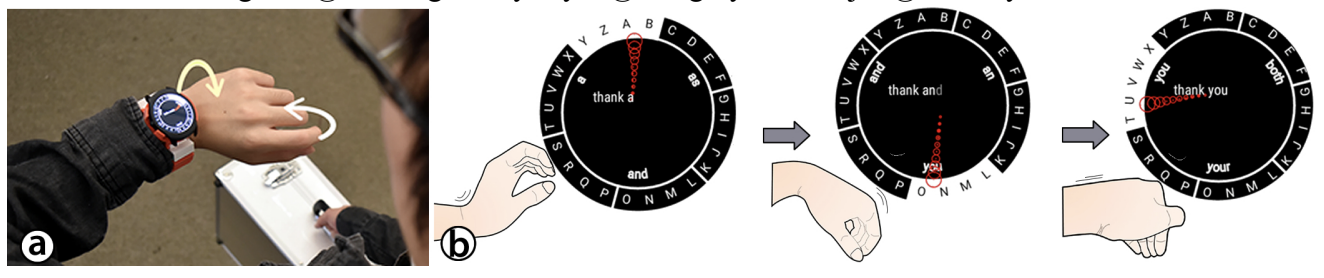
\includegraphics[width=0.6\linewidth]{wrist}
		\caption{Source: Gong et al. CHI 2018; \url{https://dl.acm.org/doi/10.1145/3173574.3173755}, downloads: \url{https://cs.dartmouth.edu/~zheer/files/WrisText.pdf}}
	\end{figure}
	
	Identify (1) Research Question, (2) Hypotheses, (3) IV and DV, (4) Order Effects, (5) Task and Procedure

	\end{block}
\end{frame}

\begin{frame}
	\frametitle{4th Workshop Solution}
	\begin{itemize}
		\item \textbf{Research Question}:  How to best design wrist-based one-handed small-form-factor text entry entry technique?  Also,  can users learn the technique?
		\item \textbf{Hypothesis}:  (1) Human performance on the wrist will determine how many directions they can perform with reasonable accuracy which will then can be further optimized in the keyboard layout (study 1),  (2) Users can master how they use the wrist after several days of training, and eventually can even perform eyes-free input (study 2)
		\item \textbf{Study 1}		
		\begin{itemize}
			\item \textbf{IV}: Target Location (8), Target Size (5) 
			\item \textbf{DV}: Time,  Accuracy,  Comfort
			\item \textbf{Participants}: 15
			\item \textbf{Apparatus}: Smartwatch, laptop
			\item \textbf{Task}: 8 location x 5 size x 5 repetitions x 15 participants
			\item \textbf{Data analysis}: ANOVA with posthoc bonferroni corrections;  questionnaires for comfort ratings
			\item \textbf{Findings}: A target size need to be at least 55.2 degree
		\end{itemize}
		
		\end{itemize}
\end{frame}

\begin{frame}
	\frametitle{Solution}
	\begin{itemize}
		\item \textbf{Study 2}:
		\begin{itemize}
			\item \textbf{IV}: Postures (hand up and down) 
			\item \textbf{DV}: Speed, Accuracy, Auto-completion rate (over 5 days)
			\item \textbf{Participants}: 10
			\item \textbf{Apparatus}: Smartwath without a ticwatch phototype; Finger-worn capacitive sensors; 27 inch screen to illustrate what input text 
			\item \textbf{Task}: 10 participants x 5 repetition x 18 trials x 2 postures
			\item \textbf{Data analysis}: ANOVA with posthoc bonferroni corrections
			\item \textbf{Findings}: User can improve through practice over time and can even perform eyes-free input with even better performance!
		\end{itemize}
	\end{itemize}
\end{frame}

\begin{frame}
\Huge{\centerline{Questions}}
\end{frame}

%----------------------------------------------------------------------------------------

\end{document} 